\documentclass{standalone}
\usepackage{tikz}
\usepackage{ctex,siunitx}
\setCJKmainfont{Noto Serif CJK SC}
\usepackage{tkz-euclide}
\usepackage{amsmath}
\usetikzlibrary{patterns, calc,3d}
\usetikzlibrary {decorations.pathmorphing,decorations.pathreplacing,decorations.shapes}
\begin{document}
\small
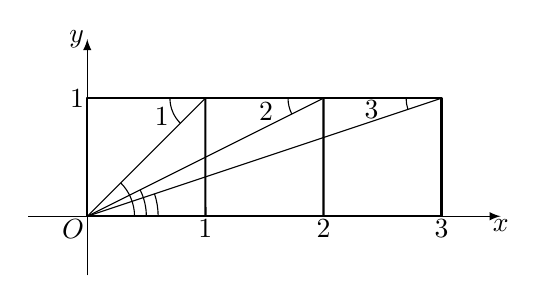
\begin{tikzpicture}[>=latex,scale=1.5,inner sep=1pt]
  \draw[->](-0.5,0)--(3.5,0)node[below]{$x$};
  \draw[->](0,-0.5)--(0,1.5)node[left]{$y$};
  \node at (0,0)[below left]{$O$};
  \tkzDefPoints{0/0/O,0/1/A,1/1/B,2/1/C,3/1/D,3/0/E}
  \tkzDrawPolygon[thick](O,A,D,E)
  \tkzDrawSegments[thin](O,B O,C O,D)
  \draw[thick](B)--(1,0)(C)--(2,0);
  \foreach \x[count=\i] in {B,C,D}
  {
    \tkzMarkAngle[size=0.3](A,\x,O)
    \tkzLabelAngle[pos={0.3+\i*0.1}](A,\x,O){$\i$}
    \tkzMarkAngle[size={0.3+\i*0.1}](E,O,\x)
    \node at (\i,0)[below]{$\i$};
  }
  \node at (0,1)[left]{$1$};
\end{tikzpicture}
\end{document}